\documentclass[usenames,dvipsnames, 18pt, compress, aspectratio=169]{beamer}

% can be compiled by xelatex -shell-escape presentation.tex
% lualatex -shell-escape presentation.tex

\usetheme[]{metropolis}

\usepackage[utf8]{inputenc}
\usepackage[russian, english]{babel}
\usepackage{booktabs}
\usepackage[scale=2]{ccicons}
\usepackage{listings}
\usepackage{marvosym}
\usepackage{color}
\usepackage{xcolor}
\usepackage[document]{ragged2e}
\usepackage[export]{adjustbox}
\usepackage{fontawesome}
\usepackage{enumitem}
\usepackage{minted}
\usemintedstyle{tango}
\usepackage[normalem]{ulem}
\usepackage{tikz}
\usetikzlibrary{patterns}
\usetikzlibrary{mindmap}
\usetikzlibrary{shapes.misc, fit}
\usepackage{graphicx}
\usepackage{eso-pic}
\usepackage{verbatim}
\usepackage{smartdiagram}
\usesmartdiagramlibrary{additions}
\usetikzlibrary{trees}
\usepackage{datetime}
\usepackage{hyperref}
\usepackage{forloop}
\usepackage{csquotes}
\usetikzlibrary{tikzmark}

\usepackage{tcolorbox}
\usepackage{tabularx}
\usepackage{array}
\usepackage{colortbl}
\tcbuselibrary{skins}

\usetikzlibrary{shapes,arrows,positioning}
\graphicspath{{images/}}
\newfontfamily{\FA}{FontAwesome}

\def\twitter{{\FA \faTwitter}}
\def\github{{\FA \faGithub}}
\def\email{{\FA \faEnvelope}}

\renewcommand{\ttdefault}{pcr}
\newfontfamily{\ttfamily}{Fira Code}

\usefonttheme{professionalfonts} % using non standard fonts for beamer
\usefonttheme{serif} % default family is serif
\usepackage{fontspec}
\setmainfont{Liberation Sans}
\newfontfamily\ExtraLight{Liberation Sans}
\newfontfamily\Light{Liberation Sans}
\newfontfamily\Book{Liberation Sans}
\newfontfamily\Medium{Liberation Sans}

\makeatletter
\newcommand\HUGE{\@setfontsize\Huge{32}{41}}
\makeatother

\newcommand\AtPagemyUpperLeft[1]{\AtPageLowerLeft{%
\put(\LenToUnit{0.85\paperwidth},\LenToUnit{0.05\paperheight}){#1}}}

\newcommand\AtPagemyUpperTop[1]{\AtPageLowerLeft{%
\put(\LenToUnit{0.42\paperwidth},\LenToUnit{0.90\paperheight}){#1}}}

\renewcommand{\ULthickness}{2.0pt}

\definecolor{links}{HTML}{0099FF}
\hypersetup{colorlinks, linkcolor=, urlcolor=links}
\definecolor{greenGood}{HTML}{99FF99}
\definecolor{redBad}{HTML}{FF9980}

\setbeamerfont{section title}{family=\Book, size=\Huge, shape=\normalfont}
\setbeamerfont{frametitle}{family=\Book, size=\large, shape=\normalfont}
\setbeamerfont{title}{family=\Book, size=\Large, shape=\normalfont}
\setbeamerfont{subtitle}{size=\small}
\setbeamerfont{author}{family=\ExtraLight, size=\footnotesize}

\definecolor{cec1d24}{RGB}{236,29,36}
\definecolor{cffffff}{RGB}{255,255,255}

\pagenumbering{gobble}

\newdateformat{specialdate}{\twodigit{\THEDAY}-\twodigit{\THEMONTH}-\THEYEAR}

%\newcommand\tikzmark[1]{%
  %\tikz[overlay,remember picture] \coordinate (#1);}

\setbeamertemplate{title page}
{

  \vspace*{2.1cm}
  \begin{minipage}[b][\paperheight]{\textwidth}
  \begin{center}

    \ifx\inserttitle\@empty\else
    {{% \inserttitle is nonempty
      \raggedright%
      %\linespread{1.0}%
      \usebeamerfont{title}%
      \usebeamercolor[fg]{title}%
      %\vspace*{1.3em}
      \if@noSmallCapitals%
        \inserttitle%
      \else%
        \scshape{\color{black} \textbf{\begin{center}\inserttitle\end{center}}}%
      \fi%
      \vspace*{0.3em}
    }}
    \fi

    \vspace*{0.5em}%

    \ifx\insertsubtitle\@empty\else
    {{% \insertsubtitle is nonempty
      \usebeamerfont{subtitle}%
      \usebeamercolor[fg]{subtitle}%
      {\color{black} \insertsubtitle}%
      \vspace*{3.0em}%
    }}
    \fi

    \vspace*{1.0em}%

    \usebeamerfont{author}%
    \usebeamercolor[fg]{author}%
    {\color{black} \insertauthor}%

    \vspace*{1.5em}
    \fontsize{8pt}{10}\selectfont
    {\color{black} 03-12-2019}%

    \vfill
    \vspace*{2em}
  \end{center}
  \end{minipage}
}

\setbeamertemplate{section page}
{
  \vspace{2em}
  \centering
  \begin{minipage}{22em}
    \usebeamercolor[fg]{section title}
    \usebeamerfont{section title}
    {\color{black} \insertsectionhead\\[-1ex]}
  \end{minipage}
  \par
}

\setbeamertemplate{footline}
{
\begin{beamercolorbox}[wd=\textwidth,ht=3ex,dp=3ex,leftskip=0.3cm,rightskip=0.3cm]{structure}
  \usebeamerfont{page number in head/foot}
  \insertframenumber
\end{beamercolorbox}
}

\title{Modern BTree\\ techniques}
\subtitle{}
\date{\today}
\author{DMITRY DOLGOV}
\institute{}

\tikzset{rum-node/.style={draw,circle,fill=white,minimum width=2cm}}
\tikzset{rum-extra-node/.style={rectangle, draw, dashed, rounded corners, fill=white }}
\tikzset{btree-key/.style={minimum height=1cm, pattern=north west lines, draw}}
\tikzset{btree-pointer/.style={minimum height=1cm, draw}}
\tikzset{btree-hide/.style={draw opacity=0, line width=0, pattern=none}}
\tikzset{btree-empty/.style={btree-pointer, dashed}}
\tikzset{btree-leaf/.style={fill=greenGood}}
\tikzset{btree-branch/.style={fill=gray!20}}
\tikzset{btree-line/.style={line width=0.5pt}}
\tikzset{btree-path/.style={btree-pointer, minimum width=0.8cm, fill=red, opacity=0.5}}
\tikzset{>=latex}
\tikzset{btree-high-key/.style={btree-key, pattern=north west lines, pattern color=red, draw=red}}
\tikzset{btree-key-prefix/.style={btree-key, minimum height=0.2cm, fill=red, opacity=0.5}}
\tikzset{btree-key-compare/.style={btree-key, minimum height=0.6cm, fill=blue, opacity=0.5}}
\tikzset{arrow-pointer/.style={
        single arrow,
        minimum height=1.5cm,
        inner sep=3pt,
        line width=1pt,
        draw,
        color=gray,
        single arrow tip angle=45,
        single arrow head extend=0.1cm
    }
}
\tikzset{btree-indirection/.style={btree-key, minimum width=0.2cm, inner sep=0, pattern=none}}
\tikzset{btree-page-header/.style={btree-key, minimum width=0.5cm, inner sep=0, pattern=none}}
\tikzset{cpu-cache/.style={draw, minimum width=1cm, minimum height=1cm, text width=1cm, align=center, rounded corners}}
\tikzset{cpu-cache-hide/.style={cpu-cache, draw=none, color=white}}

\newcommand{\btreenode}[5] {
    \path
      node[btree-pointer, #2, #3] (pointer1#1) {}
      node[btree-key, right=0 of pointer1#1, #3] (sep1#1) {}
      node[btree-key, left=0 of pointer1#1, #3] (sep2#1) {}
      node[btree-pointer, right=0 of sep1#1, #3] (pointer2#1) {}
      node[btree-pointer, left=0 of sep2#1, #3] (pointer3#1) {}
      node[btree-key, right=0 of pointer2#1, #3] (sep3#1) {}
      node[btree-key, left=0 of pointer3#1, #3] (sep4#1) {}
      node[draw, inner sep=0, behind path, #4,
          fit=(pointer1#1)(pointer2#1)(pointer3#1)
              (sep1#1)(sep2#1)(sep3#1)(sep4#1)
      ] (node#1) {};

      \ifthenelse{ \equal{#5}{show-pointers} } {
            \coordinate[below=0.5 of pointer1#1] (heap-pointer1#1);
            \coordinate[below=0.5 of pointer2#1] (heap-pointer2#1);
            \coordinate[below=0.5 of pointer3#1] (heap-pointer3#1);

            \draw[->, btree-line] (pointer1#1.south) -- (heap-pointer1#1.north);
            \draw[->, btree-line] (pointer2#1.south) -- (heap-pointer2#1.north);
            \draw[->, btree-line] (pointer3#1.south) -- (heap-pointer3#1.north);
      } {}
}

\newcounter{itemid}
\newcounter{itemid-prev}
\newcounter{itemid-next}

\newcommand{\btreenodewithitems}[5] {
    \node[btree-key, #4] (key#11) {};
    \forloop{itemid}{2}{\value{itemid} < #2} {
      \setcounter{itemid-prev}{\value{itemid} - 1}
      \ifthenelse{\number\value{itemid} < #3} {
        \node[btree-key, right=0.2cm of key#1\number\value{itemid-prev}]
          (key#1\number\value{itemid}) {};
      } {
        \node[btree-empty, right=0.2cm of key#1\number\value{itemid-prev}]
          (key#1\number\value{itemid}) {};
      }
    }
    \setcounter{itemid-prev}{\value{itemid} - 1}
    \node[btree-high-key, right=0.2cm of key#1\number\value{itemid-prev}]
        (high-key#1) {};
    \node[draw, inner sep=0.2cm, behind path, #5,
        fit=(high-key#1)\directlua{
          for index=1,#2-1 do
              tex.print("(key#1"..index..")")
          end}
    ] (node#1) {};

    %% redraw after background
    \node[btree-key, #4] (key#11) {};
    \forloop{itemid}{2}{\value{itemid} < #2} {
      \setcounter{itemid-prev}{\value{itemid} - 1}
      \ifthenelse{\number\value{itemid} < #3} {
        \node[btree-key, right=0.2cm of key#1\number\value{itemid-prev}]
          (key#1\number\value{itemid}) {};
      } {
        \node[btree-empty, right=0.2cm of key#1\number\value{itemid-prev}]
          (key#1\number\value{itemid}) {};
      }
    }
    \setcounter{itemid-prev}{\value{itemid} - 1}
    \node[btree-high-key, right=0.2cm of key#1\number\value{itemid-prev}]
        (high-key#1) {};
}

\newcommand{\btreenodewithindirectioninternal}[5] {
    \node[btree-page-header, #4] (page-header#1) {};
    \node[btree-indirection, #4, right=0.2cm of page-header#1] (indirection-key#11) {};
    \forloop{itemid}{2}{\value{itemid} < #2} {
      \setcounter{itemid-prev}{\value{itemid} - 1}
      \node[btree-indirection, right=0 of indirection-key#1\number\value{itemid-prev}]
        (indirection-key#1\number\value{itemid}) {};
    }

    \node[btree-key, #4, right=1cm of indirection-key#1\number\value{itemid-prev}] (key#11) {};
    \forloop[2]{itemid}{2}{\value{itemid} < #2} {
      \setcounter{itemid-prev}{\value{itemid} - 1}
      \setcounter{itemid-next}{\value{itemid} + 1}
      \node[btree-key, right=0.2cm of key#1\number\value{itemid-prev}, minimum width=1cm]
        (key#1\number\value{itemid}) {};
      \node[btree-key, right=0.2cm of key#1\number\value{itemid}] (key#1\number\value{itemid-next}) {};
    }
}

\newcommand{\btreenodewithindirection}[5] {
    \btreenodewithindirectioninternal{#1}{#2}{#3}{#4}{#5}
    \node[draw, inner sep=0.2cm, behind path, #5,
        fit=(page-header#1)
        \directlua{
          for index=1,#2 do
              tex.print("(key#1"..index..")")
          end}
        \directlua{
          for index=1,#2-1 do
              tex.print("(indirection-key#1"..index..")")
          end}
    ] (node#1) {};

    %% redraw after background
    \btreenodewithindirectioninternal{#1}{#2}{#3}{#4}{#5}
}

\begin{document}
{
  \usebackgroundtemplate{
\includegraphics[width=\paperwidth]{template_2.png}}%
  \fontsize{17pt}{18}\selectfont
  \maketitle
}

\AddToShipoutPictureBG{
  \AtPagemyUpperLeft{{
\includegraphics[width=2.0cm,keepaspectratio]{logo.png}}}
}%

\setbeamertemplate{background canvas}{
\begin{tikzpicture}
    \clip (0,0) rectangle (\paperwidth,\paperheight);
    \fill[color=orange] (4cm, \paperheight-6pt) rectangle (\paperwidth-4cm,\paperheight);
\end{tikzpicture}
}

\fontsize{17pt}{18}\selectfont

\begin{frame}
    \frametitle{}
    \begin{center}
        \only<1>{
            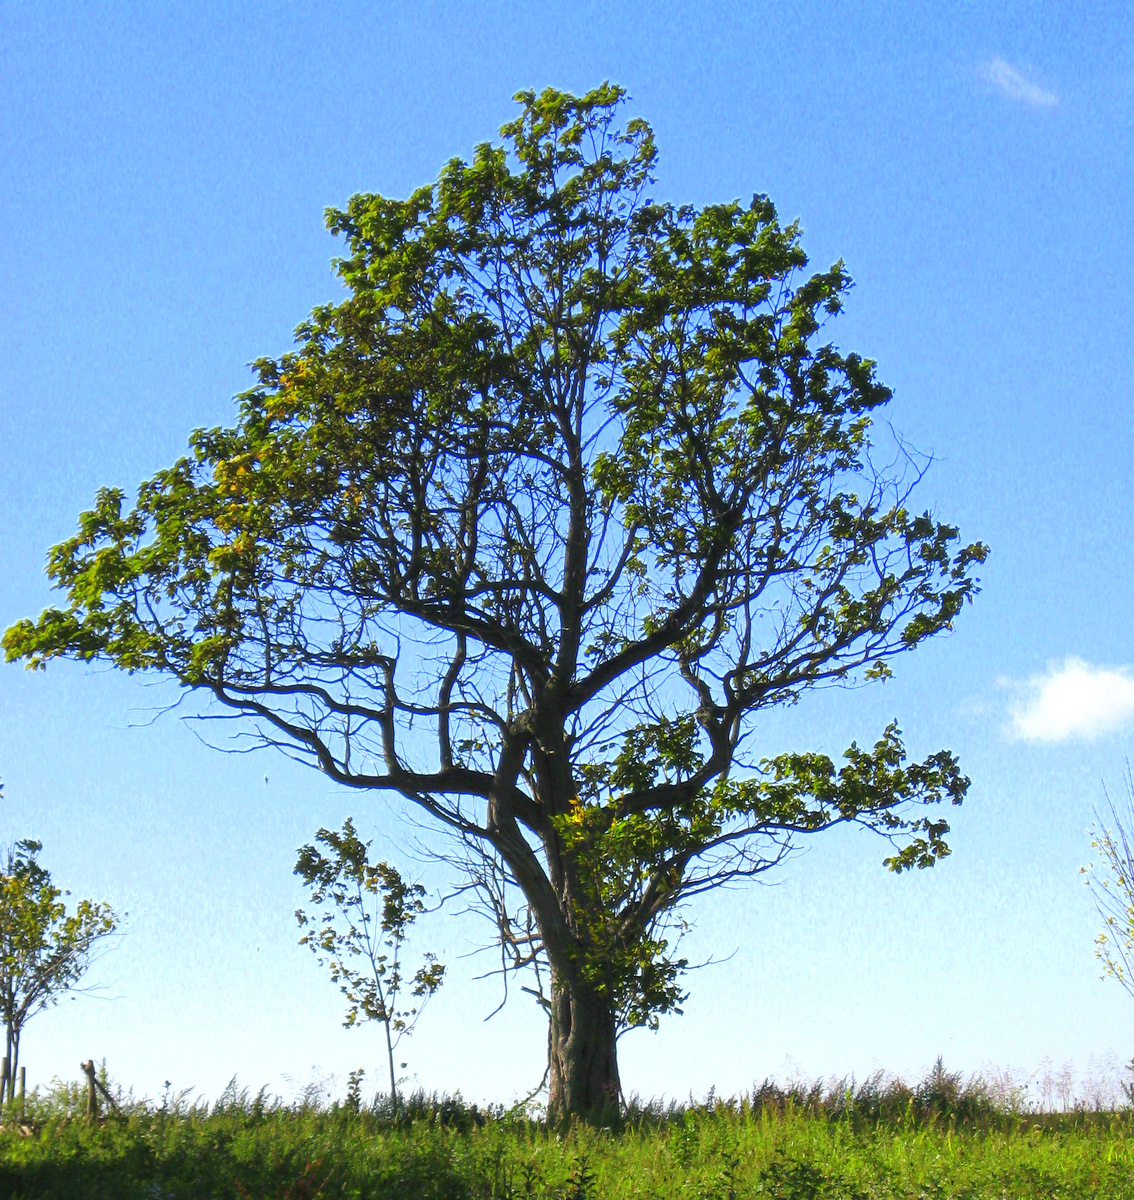
\includegraphics[width=0.5\textwidth,center]{tree.jpg}
            \vspace{-0.8cm}
            \hspace*{6cm}
            \href{https://www.flickr.com/photos/aspis7/5075169756/}
                 {\color{white}\fontsize{5pt}{0}\selectfont @aspis7}
        }
        \only<2>{
            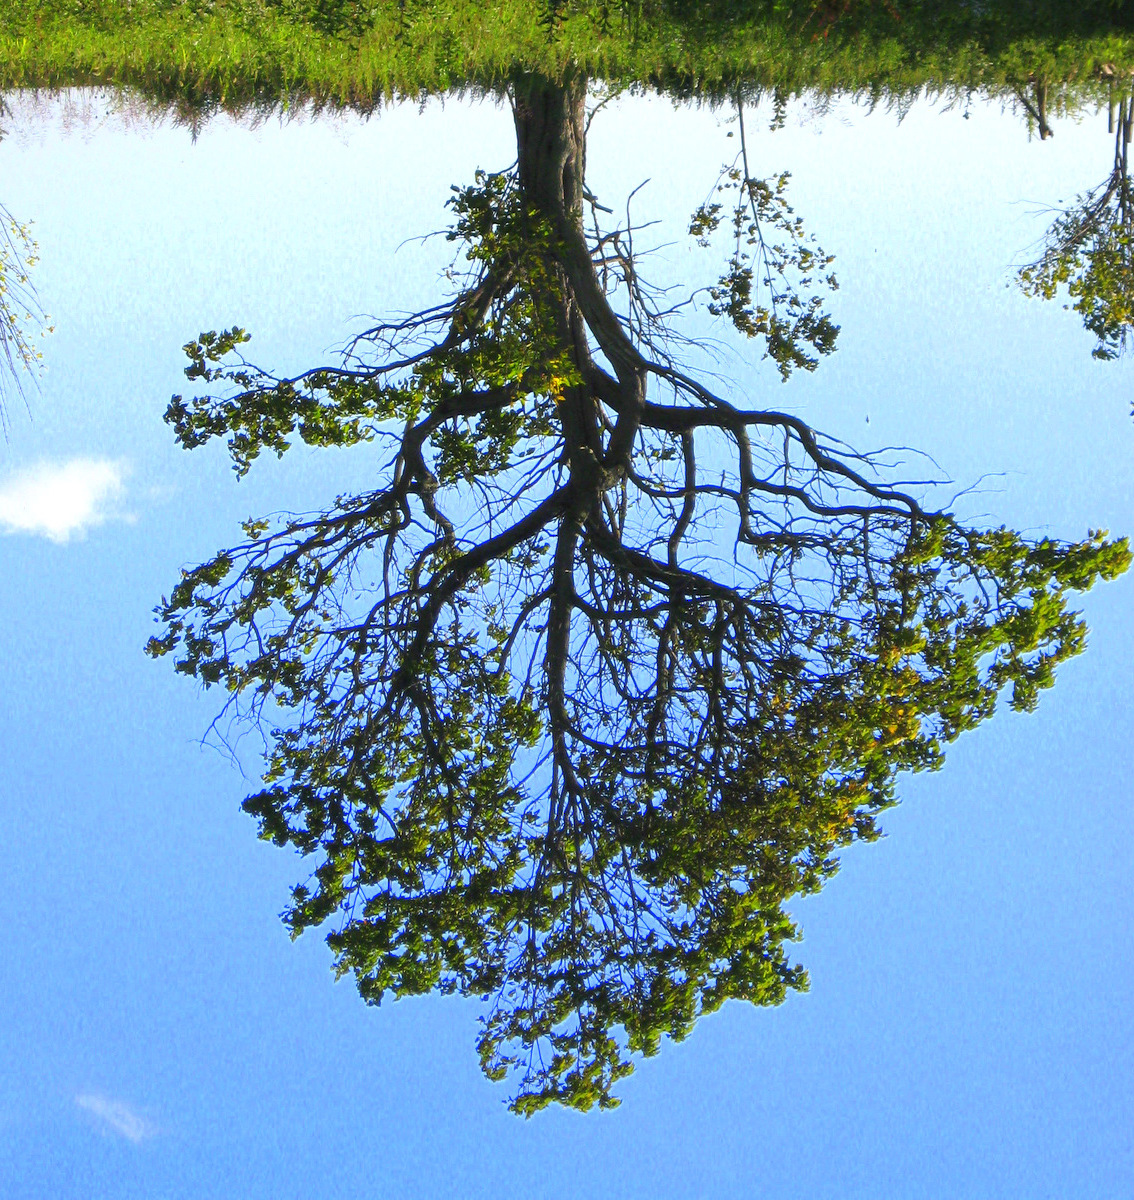
\includegraphics[width=0.5\textwidth,center]{cs_tree.jpg}
            \vspace{-0.8cm}
            \hspace*{6cm}
            \href{https://www.flickr.com/photos/aspis7/5075169756/}
                 {\color{white}\fontsize{5pt}{0}\selectfont @aspis7}
        }
    \end{center}
\end{frame}

\begin{frame}[fragile]{}
    \frametitle{}

    \begin{itemize}[label={\MVRightarrow}]
        \item <+-> D. Comet, "Ubiquitous B-tree", ACM Comp. Surv., vol. 11, no.
            2, 1979.
        \item <+-> Graefe, Goetz and Harumi A. Kuno. "Modern B-tree
            techniques." IEEE 27th International Conference on Data
            Engineering, 2011.
    \end{itemize}
\end{frame}

\begin{frame}[fragile]{}
    \frametitle{}

    \def\arraystretch{1.5}
    \begin{tabular}{cccc}
        B-Tree & B$^{+}$-Tree & B$_{link}$-Tree & DP-Tree \\
        wB$^{+}$-Tree & NV-Tree & FP-Tree & FASTFAIR \\
        HiKV & Mass-Tree & Skip List & ART \\
        WORT & CDDS-Tree & Bw-Tree & HOT \\
        KISS-Tree & VAST-Tree & FAST & HV-Tree \\
        UB-Tree & LHAM & MDM & Hybrid B$^{+}$-Tree
    \end{tabular}
\end{frame}

\begin{frame}
    \frametitle{}
    \begin{center}

    \only<1>
    {
        \begin{tikzpicture}[]
            \node [rum-node] (memory) at ( 3, 0) {Mem};
            \node [rum-node] (write) at (-3, 0) {Write};
            \node [rum-node] (read) at ( 0, 3) {Read};
            \draw (read) -- (write) -- (memory) -- (read);
            \begin{scope}[on background layer]
                \fill [gray, opacity=0.2]
                    (read.center) --
                    (write.center) --
                    (memory.center) -- cycle;
            \end{scope}
        \end{tikzpicture}
    }

    \only<2>
    {
        \begin{tikzpicture}[]
            \node [rum-node, fill=greenGood] (memory) at ( 3, 0) {Mem};
            \node [rum-node, fill=redBad] (write) at (-3, 0) {Write};
            \node [rum-node, fill=greenGood] (read) at ( 0, 3) {Read};
            \draw (read) -- (write) -- (memory) -- (read);
            \begin{scope}[on background layer]
                \fill [gray, opacity=0.2]
                    (read.center) --
                    (write.center) --
                    (memory.center) -- cycle;
            \end{scope}
        \end{tikzpicture}
    }

    \only<3>
    {
        \begin{tikzpicture}[]
            \node [rum-extra-node] (complex) at ( 0, -3) {Complexity?};
            \node [rum-node] (memory) at ( 3, 0) {Mem};
            \node [rum-node] (write) at (-3, 0) {Write};
            \node [rum-node] (read) at ( 0, 3) {Read};
            \draw (read) -- (memory) -- (complex) -- (write) -- (read);
            \begin{scope}[on background layer]
                \fill [gray, opacity=0.2]
                    (read.center) --
                    (memory.center) --
                    (complex.center) --
                    (write.center) -- cycle;
            \end{scope}
        \end{tikzpicture}
    }

    \end{center}
\end{frame}

\begin{frame}[fragile]{}
    \frametitle{}

    \begin{center}
    \textbf{B$^+$Tree}
    \vspace{1cm}

    \begin{overprint}[12cm]
        \onslide<1>
        \begin{tikzpicture}[]
            \btreenode{1}{}{btree-hide}{}{}
            \btreenode{2}{below=1cm of node1.south}{btree-hide}{}{}
            \btreenode{3}{below=1cm of node1.south west, xshift=-3cm}{btree-hide}{}{}
            \btreenode{4}{below=1cm of node1.south east, xshift=3cm}{btree-hide}{}{}

            \draw[->, btree-line] (pointer11.south) -- (pointer12.north);
            \draw[->, btree-line] (pointer21.south)
                .. controls ([yshift=-1cm] pointer21) and ([yshift=1cm] pointer14) ..
                (pointer14.north);
            \draw[->, btree-line] (pointer31.south)
                .. controls ([yshift=-1cm] pointer31) and ([yshift=1cm] pointer13) ..
                (pointer13.north);

            \coordinate[right=0.5cm of sep34.east] (link-sep34);
            \draw[btree-hide] ([yshift=0.1cm]sep34.east) -- ([yshift=0.1cm]link-sep34.west);
            \coordinate[left=0.5cm of sep43.west] (link-sep43);
            \draw[btree-hide] ([yshift=0.1cm]sep43.west) -- ([yshift=0.1cm]link-sep43.east);
        \end{tikzpicture}

        \onslide<2>
        \begin{tikzpicture}[]
            \btreenode{1}{}{btree-hide}{btree-branch}{}
            \btreenode{2}{below=1cm of node1.south}{btree-hide}{btree-leaf}{}
            \btreenode{3}{below=1cm of node1.south west, xshift=-3cm}{btree-hide}{btree-leaf}{}
            \btreenode{4}{below=1cm of node1.south east, xshift=3cm}{btree-hide}{btree-leaf}{}

            \draw[->, btree-line] (pointer11.south) -- (pointer12.north);
            \draw[->, btree-line] (pointer21.south)
                .. controls ([yshift=-1cm] pointer21) and ([yshift=1cm] pointer14) ..
                (pointer14.north);
            \draw[->, btree-line] (pointer31.south)
            .. controls ([yshift=-1cm] pointer31) and ([yshift=1cm] pointer13) ..
            (pointer13.north);

            \coordinate[right=0.5cm of sep34.east] (link-sep34);
            \draw[btree-hide] ([yshift=0.1cm]sep34.east) -- ([yshift=0.1cm]link-sep34.west);
            \coordinate[left=0.5cm of sep43.west] (link-sep43);
            \draw[btree-hide] ([yshift=0.1cm]sep43.west) -- ([yshift=0.1cm]link-sep43.east);
        \end{tikzpicture}

        \onslide<3>
        \begin{tikzpicture}[]
            \btreenode{1}{}{}{btree-branch}{}
            \btreenode{2}{below=1cm of node1.south}
                {}{btree-leaf}{show-pointers}
            \btreenode{3}{below=1cm of node1.south west, xshift=-3cm}
                {}{btree-leaf}{show-pointers}
            \btreenode{4}{below=1cm of node1.south east, xshift=3cm}
                {}{btree-leaf}{show-pointers}

            \draw[->, btree-line] (pointer11.south) -- (pointer12.north);
            \draw[->, btree-line] (pointer21.south)
                .. controls ([yshift=-1cm] pointer21) and ([yshift=1cm] pointer14) ..
                (pointer14.north);
            \draw[->, btree-line] (pointer31.south)
                .. controls ([yshift=-1cm] pointer31) and ([yshift=1cm] pointer13) ..
                (pointer13.north);

            \coordinate[right=0.5cm of sep34.east] (link-sep34);
            \draw[btree-hide] ([yshift=0.1cm]sep34.east) -- ([yshift=0.1cm]link-sep34.west);
            \coordinate[left=0.5cm of sep43.west] (link-sep43);
            \draw[btree-hide] ([yshift=0.1cm]sep43.west) -- ([yshift=0.1cm]link-sep43.east);
        \end{tikzpicture}

        \onslide<4>
        \begin{tikzpicture}[]
            \btreenode{1}{}{}{btree-branch}{}
            \btreenode{2}{below=1cm of node1.south}
                {}{btree-leaf}{show-pointers}
            \btreenode{3}{below=1cm of node1.south west, xshift=-3cm}
                {}{btree-leaf}{show-pointers}
            \btreenode{4}{below=1cm of node1.south east, xshift=3cm}
                {}{btree-leaf}{show-pointers}

            \draw[->, btree-line] (pointer11.south) -- (pointer12.north);
            \draw[->, btree-line] (pointer21.south)
                .. controls ([yshift=-1cm] pointer21) and ([yshift=1cm] pointer14) ..
                (pointer14.north);
            \draw[->, btree-line] (pointer31.south)
                .. controls ([yshift=-1cm] pointer31) and ([yshift=1cm] pointer13) ..
                (pointer13.north);

            \draw[->, btree-line] ([yshift=0.1cm]sep33.east) -- ([yshift=0.1cm]sep42.west);
            \draw[->, btree-line] ([yshift=0.1cm]sep32.east) -- ([yshift=0.1cm]sep44.west);
            \coordinate[right=0.5cm of sep34.east] (link-sep34);
            \draw[->, btree-line] ([yshift=0.1cm]sep34.east) -- ([yshift=0.1cm]link-sep34.west);
            \coordinate[left=0.5cm of sep43.west] (link-sep43);
            \draw[btree-hide] ([yshift=0.1cm]sep43.west) -- ([yshift=0.1cm]link-sep43.east);
        \end{tikzpicture}

        \onslide<5>
        \begin{tikzpicture}[]
            \btreenode{1}{}{}{btree-branch}{}
            \btreenode{2}{below=1cm of node1.south}
                {}{btree-leaf}{show-pointers}
            \btreenode{3}{below=1cm of node1.south west, xshift=-3cm}
                {}{btree-leaf}{show-pointers}
            \btreenode{4}{below=1cm of node1.south east, xshift=3cm}
                {}{btree-leaf}{show-pointers}

            \draw[->, btree-line] (pointer11.south) -- (pointer12.north);
            \draw[->, btree-line] (pointer21.south)
                .. controls ([yshift=-1cm] pointer21) and ([yshift=1cm] pointer14) ..
                (pointer14.north);
            \draw[->, btree-line] (pointer31.south)
                .. controls ([yshift=-1cm] pointer31) and ([yshift=1cm] pointer13) ..
                (pointer13.north);

            \draw[->, btree-line] ([yshift=0.1cm]sep33.east) -- ([yshift=0.1cm]sep42.west);
            \draw[->, btree-line] ([yshift=0.1cm]sep32.east) -- ([yshift=0.1cm]sep44.west);
            \draw[<-, btree-line] ([yshift=-0.1cm]sep33.east) -- ([yshift=-0.1cm]sep42.west);
            \draw[<-, btree-line] ([yshift=-0.1cm]sep32.east) -- ([yshift=-0.1cm]sep44.west);
            \coordinate[right=0.5cm of sep34.east] (link-sep34);
            \draw[->, btree-line] ([yshift=0.1cm]sep34.east) -- ([yshift=0.1cm]link-sep34.west);
            \coordinate[left=0.5cm of sep43.west] (link-sep43);
            \draw[->, btree-line] ([yshift=0.1cm]sep43.west) -- ([yshift=0.1cm]link-sep43.east);
        \end{tikzpicture}

        \onslide<6>
        \begin{tikzpicture}[]
            \btreenode{1}{}{}{btree-branch}{}
            \btreenode{2}{below=1cm of node1.south}
                {}{btree-leaf}{show-pointers}
            \btreenode{3}{below=1cm of node1.south west, xshift=-3cm}
                {}{btree-leaf}{show-pointers}
            \btreenode{4}{below=1cm of node1.south east, xshift=3cm}
                {}{btree-leaf}{show-pointers}

            \draw[->, btree-line, color=red, line width=2pt] (pointer11.south) -- (pointer12.north);
            \draw[->, btree-line] (pointer21.south)
                .. controls ([yshift=-1cm] pointer21) and ([yshift=1cm] pointer14) ..
                (pointer14.north);
            \draw[->, btree-line] (pointer31.south)
                .. controls ([yshift=-1cm] pointer31) and ([yshift=1cm] pointer13)
                .. (pointer13.north);

            \path
              node[btree-path, below=-0.505 of pointer11.west] (path-pointer1) {}
              node[btree-path, below=-0.505 of pointer32.west] (path-pointer2) {};

            \draw[->, btree-line, color=red, line width=2pt]
                (pointer32.south) -- (heap-pointer32.north);

            \draw[->, btree-line] ([yshift=0.1cm]sep33.east) -- ([yshift=0.1cm]sep42.west);
            \draw[->, btree-line] ([yshift=0.1cm]sep32.east) -- ([yshift=0.1cm]sep44.west);
            \draw[<-, btree-line] ([yshift=-0.1cm]sep33.east) -- ([yshift=-0.1cm]sep42.west);
            \draw[<-, btree-line] ([yshift=-0.1cm]sep32.east) -- ([yshift=-0.1cm]sep44.west);
            \coordinate[right=0.5cm of sep34.east] (link-sep34);
            \draw[->, btree-line] ([yshift=0.1cm]sep34.east) -- ([yshift=0.1cm]link-sep34.west);
            \coordinate[left=0.5cm of sep43.west] (link-sep43);
            \draw[->, btree-line] ([yshift=0.1cm]sep43.west) -- ([yshift=0.1cm]link-sep43.east);
        \end{tikzpicture}
    \end{overprint}
    \end{center}


    \linespread{0.5}
    \vspace{0.5cm}
    \color{black}\fontsize{6pt}{0}\selectfont
        P. Lehman and S. Yao, Efficient Locking for Concurrent Operations on B-Trees, ACM Transactions on Database Systems, Vol 6, No. 4, December 1981, pp 650-670
    \linespread{1.5}

\end{frame}
\note{
    Postgres uses variation of B-link Tree, seems like MySQL innodb uses
    regular B+ Tree.
}

\fontsize{17pt}{18}\selectfont
\begin{frame}[fragile]{}
    \frametitle{}

    \begin{center}
    \textbf{Page split}
    \vspace{1cm}

    \begin{overprint}[8cm]
        \onslide<1>
        \begin{tikzpicture}[]
            \btreenodewithitems{1}{5}{2}{}{btree-branch}
            \btreenodewithitems{2}{5}{4}{below=1cm of key11, xshift=-2cm}{btree-leaf}
            \draw[->, btree-line] (node1.south)
                .. controls ([yshift=-1cm] node1) and ([yshift=1.2cm] node2) ..
                (node2.north);
        \end{tikzpicture}

        \onslide<2>
        \begin{tikzpicture}[]
            \btreenodewithitems{1}{5}{2}{}{btree-branch}
            \btreenodewithitems{2}{5}{4}{below=1cm of key11, xshift=-2cm}{btree-leaf}
            \draw[->, btree-line] (node1.south)
                .. controls ([yshift=-1cm] node1) and ([yshift=1.2cm] node2) ..
                (node2.north);

            \node[btree-key, below=1cm of key23] (new-key) {};
            \draw[->, btree-line] (new-key.east)
                .. controls ([xshift=1cm] new-key) and (key24) ..
                (key24.center);
        \end{tikzpicture}

        \onslide<3>
        \begin{tikzpicture}[]
            \btreenodewithitems{1}{5}{2}{}{btree-branch}
            \btreenodewithitems{2}{5}{3}{below=1cm of key11, xshift=-2cm}{btree-leaf}
            \btreenodewithitems{3}{5}{3}{below=1cm of key11, xshift=2cm}{btree-leaf}
            \draw[->, btree-line] (node1.south)
                .. controls ([yshift=-1cm] node1) and ([yshift=1.2cm] node2) ..
                (node2.north);
            \draw[->, btree-line] (node1.south)
                .. controls ([yshift=-1cm] node1) and ([yshift=1.2cm] node3) ..
                (node3.north);
        \end{tikzpicture}

        \onslide<4>
        \begin{tikzpicture}[]
            \btreenodewithitems{1}{5}{2}{}{btree-branch}
            \btreenodewithitems{2}{5}{3}{below=1cm of key11, xshift=-2cm}{btree-leaf}
            \btreenodewithitems{3}{5}{3}{below=1cm of key11, xshift=2cm}{btree-leaf}
            \draw[->, btree-line] (node1.south)
                .. controls ([yshift=-1cm] node1) and ([yshift=1.2cm] node2) ..
                (node2.north);
            \draw[->, btree-line] (node1.south)
                .. controls ([yshift=-1cm] node1) and ([yshift=1.2cm] node3) ..
                (node3.north);

            \node[btree-key, below=-0.5cm of key13.center] (promoted) {};
            \draw[->, btree-line] (key31.west)
                .. controls ([xshift=-1cm] key31) and (promoted) ..
                (promoted.center);
        \end{tikzpicture}

    \end{overprint}
    \end{center}

\end{frame}

\begin{frame}[fragile]{}
    \frametitle{}

    \begin{center}
    \textbf{Page merge}
    %\vspace{1cm}
    \end{center}

    \begin{flushleft}
        \begin{displayquote}
            "By adding periodic rebuilding of the tree, we obtain a data
            structure that is theoreticaly superior to standard B-trees in many
            ways. Our results suggest that rebalancing on deletion no only
            unnecessary but may be harmful."
        \end{displayquote}
        \footnotesize{S. Sen and R. E. Tarjan, "Deletion without rebalancing in multiway
        search trees." ISAAC, pp. 832-841, 2009}
    \end{flushleft}

\end{frame}
\note{
    Postgres deletes via marking a tuple as dead, and then vacuuming either a
    table of a single page.
}

\begin{frame}[fragile]{}
    \frametitle{}

    \begin{center}
    \begin{overprint}[8cm]
        \onslide<1>
        \begin{tikzpicture}[]
            \node [rum-node] (memory) at ( 3, 0) {Mem};
            \node [rum-node] (write) at (-3, 0) {Write};
            \node [rum-node] (read) at ( 0, 3) {Read};
            \draw (read) -- (write) -- (memory) -- (read);
            \begin{scope}[on background layer]
                \fill [gray, opacity=0.2]
                    (read.center) --
                    (write.center) --
                    (memory.center) -- cycle;
            \end{scope}

            \coordinate[below=0.5 of read] (btree-pointer);
            \coordinate[right=2 of read] (btree-angle);
            \node[above=0.5 of btree-angle, draw=none, color=white] (btree) {B-Tree};
        \end{tikzpicture}

        \onslide<2>
        \begin{tikzpicture}[]
            \node [rum-node] (memory) at ( 3, 0) {Mem};
            \node [rum-node] (write) at (-3, 0) {Write};
            \node [rum-node] (read) at ( 0, 3) {Read};
            \draw (read) -- (write) -- (memory) -- (read);
            \begin{scope}[on background layer]
                \fill [gray, opacity=0.2]
                    (read.center) --
                    (write.center) --
                    (memory.center) -- cycle;
            \end{scope}

            \coordinate[below=0.5 of read] (btree-pointer);
            \coordinate[right=2 of read] (btree-angle);
            \node[above=0.5 of btree-angle, draw=none] (btree) {B-Tree};
            \draw[->, line width=2pt] (btree)
                .. controls ([yshift=-2cm] btree) and (btree-pointer) ..
                (btree-pointer);
        \end{tikzpicture}

        \onslide<3>
        \begin{tikzpicture}[]
            \node [rum-node, fill=greenGood] (memory) at ( 3, 0) {Mem};
            \node [rum-node, fill=greenGood] (write) at (-3, 0) {Write};
            \node [rum-node, fill=redBad] (read) at ( 0, 3) {Read};
            \draw (read) -- (write) -- (memory) -- (read);
            \begin{scope}[on background layer]
                \fill [gray, opacity=0.2]
                    (read.center) --
                    (write.center) --
                    (memory.center) -- cycle;
            \end{scope}

            \coordinate[below=0.5 of read] (btree-pointer);
            \coordinate[right=2 of read] (btree-angle);
            \node[above=0.5 of btree-angle, draw=none] (btree) {B-Tree};
            \draw[->, line width=2pt] (btree)
                .. controls ([yshift=-2cm] btree) and (btree-pointer) ..
                (btree-pointer);
        \end{tikzpicture}
    \end{overprint}
    \end{center}
\end{frame}

\begin{frame}[fragile]{}
    \frametitle{}

    \begin{center}
    \textbf{Key normalization}
    \vspace{1cm}

    \begin{tabular}{cccl}
        1 & "Dirk" & "Bart" &
            \colorbox{BurntOrange}{1}
            \colorbox{SpringGreen}{0..01}
            \colorbox{BurntOrange}{1}
            \colorbox{SpringGreen}{11..00}
            \colorbox{Gray!40}{$\emptyset$}
            \colorbox{BurntOrange}{1}
            \colorbox{SpringGreen}{10..10}
            \colorbox{Gray!40}{$\emptyset$} \\
        2 & "Todd" & Null &
            \colorbox{BurntOrange}{1}
            \colorbox{SpringGreen}{0..10}
            \colorbox{BurntOrange}{1}
            \colorbox{SpringGreen}{01..00}
            \colorbox{Gray!40}{$\emptyset$}
            \colorbox{BurntOrange}{0} \\
        Null & "" & Null &
            \colorbox{BurntOrange}{0}
            \colorbox{BurntOrange}{1}
            \colorbox{Gray!40}{$\emptyset$}
            \colorbox{BurntOrange}{0} \\
    \end{tabular}

    \linespread{0.5}
    \vspace{0.5cm}
    \color{black}\fontsize{6pt}{0}\selectfont
        R. C. Singleton, "An efficient algorithm for sorting with minimal
        storage", Communications of the ACM, vol. 12, no.3 pp. 185-186, 1969
    \linespread{1.5}

    \end{center}
\end{frame}
\note{
    https://wiki.postgresql.org/wiki/Key_normalization

    Should be not used for leaves, since normalization looses the information.
    Other option is too store both normalized and original key values.
}

\begin{frame}[fragile]{}
    \frametitle{}

    \begin{center}
    \textbf{Prefix truncation}
    \vspace{1cm}

    \begin{overprint}[8cm]
        \onslide<1>
        \begin{tabular}{lll}
            & & \\
            & Smith Jack & 01-02-2019 \\
            & Smith Jane & 02-03-2019 \\
            & Smith James & 03-04-2019 \\
        \end{tabular}

        \onslide<2>
        \begin{tabular}{lll}
            & & \\
            & \colorbox{BurntOrange}{Smith Ja}ck & 01-02-2019 \\
            & \colorbox{BurntOrange}{Smith Ja}ne & 02-03-2019 \\
            & \colorbox{BurntOrange}{Smith Ja}mes & 03-04-2019 \\
        \end{tabular}

        \onslide<3>
        \begin{tabular}{lll}
            \colorbox{BurntOrange}{Smith Ja} & & \\
            & ck & 01-02-2019 \\
            & ne & 02-03-2019 \\
            & mes & 03-04-2019 \\
        \end{tabular}

        \onslide<4>
        \begin{center}
        \begin{tikzpicture}[]
            \btreenodewithitems{1}{8}{5}{}{btree-leaf}
            \coordinate[below=1cm of key11] (start1);
            \coordinate[below=1cm of high-key1] (start2);
            \draw[->, btree-line, line width=1.5pt, shorten >= 2mm] (start1) -- (key11);
            \draw[->, btree-line, line width=1.5pt, shorten >= 2mm] (start2) -- (high-key1);
        \end{tikzpicture}
        \end{center}

        \onslide<5>
        \begin{center}
        \begin{tikzpicture}[]
            \btreenodewithitems{1}{8}{5}{}{btree-leaf}
            \foreach \i in {1,...,4}
            {
                \coordinate[below=1cm of key1\i] (start\i);
                \draw[->, btree-line, line width=1.5pt, shorten >= 2mm] (start\i) -- (key1\i);
            }
        \end{tikzpicture}
        \end{center}

    \end{overprint}

    \end{center}
\end{frame}
\note{
    BerkleyDB, https://web.stanford.edu/class/cs276a/projects/docs/berkeleydb/api_c/db_set_bt_prefix.html

    TODO: mark shared parts of keys in both situations
}

\begin{frame}[fragile]{}
    \frametitle{}

    \begin{center}
    \textbf{Dynamic prefix truncation}
    \vspace{1cm}

    \begin{overprint}[8cm]
        \onslide<1>
        \begin{center}
        \begin{tikzpicture}[]
            \btreenodewithitems{1}{8}{5}{}{btree-leaf}
            \node[btree-key, below=1cm of key13.center] (compared) {};
        \end{tikzpicture}
        \end{center}

        \onslide<2>
        \begin{center}
        \begin{tikzpicture}[]
            \btreenodewithitems{1}{8}{5}{}{btree-leaf}
            \node[btree-key, below=1cm of key13.center] (compared) {};

            \node[btree-key-prefix, below=1cm of key13.center] (compared-prefix) {};
            \node[btree-key-prefix, below=-0.5cm of high-key1.center] (compared-high-key-prefix) {};
            \node[btree-key-prefix, below=-0.5cm of key11.center] (compared-first-key-prefix) {};
        \end{tikzpicture}
        \end{center}

        \onslide<3>
        \begin{center}
        \begin{tikzpicture}[]
            \btreenodewithitems{1}{8}{5}{}{btree-leaf}
            \node[btree-key, below=1cm of key13.center] (compared) {};

            \node[btree-key-prefix, below=1cm of key13.center] (compared-prefix) {};
            \node[btree-key-prefix, below=-0.5cm of high-key1.center] (compared-high-key-prefix) {};
            \node[btree-key-prefix, below=-0.5cm of key11.center] (compared-first-key-prefix) {};

            \node[btree-key-compare, below=-0.1cm of compared.center] (compare-key) {};
            \foreach \i in {1,...,4}
            {
                \node[btree-key-compare, below=-0.1cm of key1\i.center] (compare-\i) {};
            }
        \end{tikzpicture}
        \end{center}

    \end{overprint}

    \end{center}
\end{frame}

\begin{frame}[fragile]{}
    \frametitle{}

    \begin{center}
    \textbf{Suffix truncation}
    \vspace{1cm}

    \begin{overprint}[8cm]
        \onslide<1>
        \begin{tabular}{lll}
            & Johnson David & 04-02-2019 \\
            & Miller Kevin & 01-02-2019 \\
            & Miller Ned & 02-03-2019 \\
            & Miller Steven & 03-04-2019 \\
            & Smith Jack & 01-02-2019 \\
        \end{tabular}

        \onslide<2>
        \begin{tabular}{lll}
            & Johnson David & 04-02-2019 \\
            & Miller Kevin & 01-02-2019 \\
            & \tikzmark{middle}Miller Ned & 02-03-2019 \\
            & Miller Steven & 03-04-2019 \\
            & Smith Jack & 01-02-2019 \\
        \end{tabular}
        \begin{tikzpicture}[overlay, remember picture]
            \node[arrow-pointer, left=0.5cm of {pic cs:middle}, yshift=0.2cm] {};
        \end{tikzpicture}

        \onslide<3>
        \begin{tabular}{lll}
            & Johnson David & 04-02-2019 \\
            & Miller Kevin & 01-02-2019 \\
            & \tikzmark{middle}\colorbox{BurntOrange}{Miller N}ed & 02-03-2019 \\
            & Miller Steven & 03-04-2019 \\
            & Smith Jack & 01-02-2019 \\
        \end{tabular}
        \begin{tikzpicture}[overlay, remember picture]
            \node[arrow-pointer, left=0.5cm of {pic cs:middle}, yshift=0.2cm] {};
        \end{tikzpicture}

        \onslide<4>
        \begin{tabular}{lll}
            & \tikzmark{middle}\colorbox{BurntOrange}{J}ohnson David & 04-02-2019 \\
            & Miller Kevin & 01-02-2019 \\
            & Miller Ned & 02-03-2019 \\
            & Miller Steven & 03-04-2019 \\
            & Smith Jack & 01-02-2019 \\
        \end{tabular}
        \begin{tikzpicture}[overlay, remember picture]
            \node[arrow-pointer, left=0.5cm of {pic cs:middle}, yshift=0.2cm] {};
        \end{tikzpicture}

    \end{overprint}

    \linespread{0.5}
    \vspace{0.5cm}
    \color{black}\fontsize{6pt}{0}\selectfont
        R. Bayer, K. Unterauer, "Prefix B-trees", ACM Transactions on Database
        Systems, vol. 2, no. 1, pp. 11-26, 1977
    \linespread{1.5}

    \end{center}
\end{frame}
\note{
    Not a normalized version, but whole column version is in PG12
}

\begin{frame}[fragile]{}
    \frametitle{}

    \begin{center}
    \textbf{Indirection vector}
    \vspace{1cm}

    \begin{overprint}[8cm]
        \onslide<1>
        \begin{center}
        \begin{tikzpicture}[]
            \btreenodewithindirection{1}{5}{5}{}{btree-leaf}

            \foreach \i/ \shift in {1/0.35cm,2/0.11cm,3/-0.07cm,4/-0.3cm} {
                \draw[->, btree-line] ([yshift=\shift]indirection-key1\i.east) -- ([yshift=\shift]key1\i.center);
            }
          \linespread{0.5}
          \node[cpu-cache-hide, below=1cm of indirection-key12.east]
              (cpu-cache) {\footnotesize{CPU\\Cache}};

          \coordinate[above=2cm of cpu-cache.north east] (cpu-cache-top-left);
          \coordinate[above=2cm of cpu-cache.north west] (cpu-cache-top-right);
          \draw[draw=none] ([xshift=-0.2cm]cpu-cache.north east) -- ([xshift=-0.2cm]cpu-cache-top-left);
          \draw[draw=none] ([xshift=0.2cm]cpu-cache.north west) -- ([xshift=0.2cm]cpu-cache-top-right);

          \linespread{1.5}

        \end{tikzpicture}
        \end{center}

        \onslide<2>
        \begin{center}
        \begin{tikzpicture}[]
            \btreenodewithindirection{1}{5}{5}{}{btree-leaf}

            \foreach \i/ \shift/ \letter in {1/-0.6cm/a,2/-0.4cm/b,3/-0.2cm/c,4/-0.0cm/d} {
              \node[draw=none, below=\shift of indirection-key1\i.center]
                (normalized-indirection-key1\i) {\tiny{\letter}};
            }

            \foreach \i/ \shift in {1/0.35cm,2/0.11cm,3/-0.07cm,4/-0.3cm} {
                \draw[->, btree-line] ([yshift=\shift]indirection-key1\i.east) -- ([yshift=\shift]key1\i.center);
            }

          \linespread{0.5}
          \node[cpu-cache-hide, below=1cm of indirection-key12.east]
              (cpu-cache) {\footnotesize{CPU\\Cache}};

          \coordinate[above=2cm of cpu-cache.north east] (cpu-cache-top-left);
          \coordinate[above=2cm of cpu-cache.north west] (cpu-cache-top-right);
          \draw[draw=none] ([xshift=-0.2cm]cpu-cache.north east) -- ([xshift=-0.2cm]cpu-cache-top-left);
          \draw[draw=none] ([xshift=0.2cm]cpu-cache.north west) -- ([xshift=0.2cm]cpu-cache-top-right);

          \linespread{1.5}

        \end{tikzpicture}
        \end{center}

        \onslide<3>
        \begin{center}
        \begin{tikzpicture}[]
            \btreenodewithindirection{1}{5}{5}{}{btree-leaf}

            \foreach \i/ \shift/ \letter in {1/-0.6cm/a,2/-0.4cm/b,3/-0.2cm/c,4/-0.0cm/d} {
              \node[draw=none, below=\shift of indirection-key1\i.center]
                (normalized-indirection-key1\i) {\tiny{\letter}};
            }

            \foreach \i/ \shift in {1/0.35cm,2/0.11cm,3/-0.07cm,4/-0.3cm} {
                \draw[->, btree-line] ([yshift=\shift]indirection-key1\i.east) -- ([yshift=\shift]key1\i.center);
            }

          \linespread{0.5}
          \node[cpu-cache, below=1cm of indirection-key12.east]
              (cpu-cache) {\footnotesize{CPU\\Cache}};

          \coordinate[above=2cm of cpu-cache.north east] (cpu-cache-top-left);
          \coordinate[above=2cm of cpu-cache.north west] (cpu-cache-top-right);
          \draw[dashed] ([xshift=-0.2cm]cpu-cache.north east) -- ([xshift=-0.2cm]cpu-cache-top-left);
          \draw[dashed] ([xshift=0.2cm]cpu-cache.north west) -- ([xshift=0.2cm]cpu-cache-top-right);

          \linespread{1.5}

        \end{tikzpicture}
        \end{center}
    \end{overprint}

    \linespread{0.5}
    \vspace{0.5cm}
    \color{black}\fontsize{6pt}{0}\selectfont
        G. Graefe, Per-Ake Larson, "B-tree indexes and CPU caches",
        International Conference on Data Engineering, pp. 349-358, 2001
    \linespread{1.5}

    \end{center}
\end{frame}

\begin{frame}[fragile]{}
    \frametitle{}

    \begin{center}
    \textbf{SB-tree}
    \vspace{1cm}

    \begin{overprint}[8cm]
    \end{overprint}

    \end{center}
\end{frame}

\fontsize{18pt}{18}\selectfont
\begin{frame}
  \vspace*{2.5cm}
  \begin{minipage}[b][\paperheight]{\textwidth}
  \begin{center}

      %\raggedright%
      \linespread{1.0}%
      \usebeamerfont{title}%
      \usebeamercolor[fg]{title}%
      \if@noSmallCapitals%
        Questions?
      \else%
        \scshape{\color{black} Questions?}%
      \fi%
      \vspace*{0.3em}

      \usebeamerfont{subtitle}%
      \fontsize{13pt}{14}\selectfont
      \usebeamercolor[fg]{subtitle}%
        \begin{itemize}[label={}]
            \item {\color{black} \twitter\ @erthalion}
            \item {\color{black} \email\ dmitrii.dolgov at zalando dot de}
            \item {\color{black} \email\ 9erthalion6 at gmail dot com}
        \end{itemize}
      \vspace*{2.5em}%

    \vfill
    \vspace*{2em}
  \end{center}
  \end{minipage}

\end{frame}
\note{
    ClickHouse - B-Tries
}

\end{document}
